\chapter{Optimization}

\section{Introduction to Optimization}

High Performance Computing (HPC) requires extracting maximum effectiveness from code on available hardware. Optimization is thus essential, though both "optimization" and "effectiveness" are context-dependent concepts.

There is no universally "optimal" code, as optimality varies based on specific requirements and constraints. In HPC, optimization encompasses several competing dimensions:

\begin{itemize}
    \item \textbf{Memory constraints:} Minimizing memory footprint for both data structures and executable code, especially in resource-limited environments.
    
    \item \textbf{I/O constraints:} Efficient input/output operations across various media, critical for data-intensive applications where I/O bottlenecks limit performance.
    
    \item \textbf{Time constraints:} Reducing time-to-solution, whether optimizing for worst-case scenarios, average performance, or specific use cases.
    
    \item \textbf{Robustness:} Ensuring reliability and fault tolerance for mission-critical applications, sometimes at the expense of raw speed.
    
    \item \textbf{Energy constraints:} Minimizing power consumption, particularly important for large-scale HPC installations and power-limited systems.
\end{itemize}

This multidimensional nature creates inherent trade-offs between performance aspects. The fundamental challenge lies in determining which dimensions are most important for a specific application and finding an appropriate balance among competing objectives.

\begin{tipsblock}[Premature Optimization]
    \begin{center}
    \textit{Premature optimization is the root of all evil.}
    \end{center}
    \phantom{ } \hfill \textit{\textasciitilde Donald Knuth}
\end{tipsblock}

\subsection{First steps to consider}

- Dryness: Do not add unnecessary code nor duplicate code. This will make the code more difficult to maintain and debug.

- Readibility: Make the code as readable as possible. Write comments and use meaningful variable names.

- Test is part of the design:
    - unit test: separately stress each unit of the code;
    - integration test: stress the integrated behavior of all the units together;
    - system test: stress the system as a whole.

- Validation and verification are part of the design:
    - Validation ensures that the code does what it was meant to do (all modules are designed accordingly to design specifications)

    - Verification ensures that the code does what it does correctly (black-box testing against test-cases, ...)

\subsection{Compiler optimization}

Compilers are those tools that translate the code you write into machine code that the computer can understand. 

Compilers are also able to perform \textbf{sophisticated analysis} of the source code so that to produce a target code (usually an assembly code) which is \textbf{highly optimized for a given target architecture}.

- write non-obfuscated code
- design a good data structure layout
- design a “good” workflow
- take advantage of the modern out-of-order, super-scalar, multi-core architectures

\subsubsection{Optimization levels}

It is not granted that -O3, although often generating a faster code, is what you really need.

For instance, sometimes expensive optimizations may generate more code that on some architecture (e.g. with smaller caches) run slower, and using -Os may bring surprising results.

Take into accounts that modern compilers allow for local specific optimizations or compilation flags

\subsubsection{Compile for specific CPU model}

The compiler knows the architecture it is compiling on, of course. However, it will generate a portable code , i.e. a code that can run on any cpu belonging to that class of architecture.

Example: x86\_64, x86\_32, ARM, POWER9, are all classes of architecture

Besides a general set of instructions that all the cpus of a given class can understand, specific models have specific different ISA that are not compatible with others (normally you have back-compatibility).

Using appropriate switch (in gcc \texttt{-march=native -mtune=native}, in icc texttt{-xHost}), the compiler will optimize for exactly the specific cpu it’s running on, much probably producing a more performant code for it

... automatic profiling ... 
... memory allocation ... 
... C-specific hints ...

Memory aliasing:

\begin{codeblock}[language = C]
void func1 (int *a, int *b)  {
    *a += *b;
    *a += *b;
}

void func2 (int *a, int *b)  {
    *a += 2 * *b;
}
\end{codeblock}

An incautious analysis may conclude that a compiler, or even a programmer, should immediately transform func1() into func2() because, having three less memory references, it should yield to a better assembly code.

However, is it really true that the two functions behave exactly the same way in all possible conditions?

What if a = b, i.e. if a and b points to the same memory location?

The compiler can not optimize the access to a and b because it can not assume that a and b are pointing to the same memory locations or, in general, that the references will never overlap.

That is called aliasing, formally forbidden in FORTRAN: which is the reason why in some cases fortran may compile in faster executables without you paying any attention

Help your C compiler in doing the best effort, either writing a clean code or using restrict or using \texttt{-fstrict-aliasing -Wstrict-aliasing} options.

\begin{codeblock}[language = C]
void my_function (double *restrict a, double *restrict b)  {
    *a += *b;
    *a += *b;
}
\end{codeblock}

Now you’re telling the compiler that the memory regions referenced by a and b will never overlap.

So, it will feel confident in optimizing the memory accesses as much as it can (basically avoiding to re-read locations)

\section{Single core optimization}

Modern CPU architecture has evolved significantly to address performance challenges, fundamentally changing optimization approaches. As CPUs have dramatically outpaced memory speed, memory access has become a critical bottleneck, leading to the development of hierarchical memory systems that leverage data locality principles to reduce latency. Concurrently, CPUs have adopted super-scalar designs with out-of-order execution capabilities, enabling multiple operations to execute simultaneously (Instruction-Level Parallelism or ILP), provided code is appropriately structured. Operations are now broken into smaller pipelined stages to increase throughput, though these pipelines remain vulnerable to data and control hazards that can cause performance-degrading stalls. Branch predictors have become crucial front-end components that minimize pipeline disruptions from control flow changes. Additionally, modern processors incorporate vector processing through SIMD (Same Instruction Multiple Data) registers, enabling Data-Level Parallelism where a single instruction operates on multiple data elements simultaneously. However, not all computational patterns can benefit from vectorization, as this depends on data independence and access patterns.

The energy and power are a major design issue: We have seen that the power required per transistor is:

$$
C\times V^2 \times f
$$

\begin{figure}[H]
    \centering
    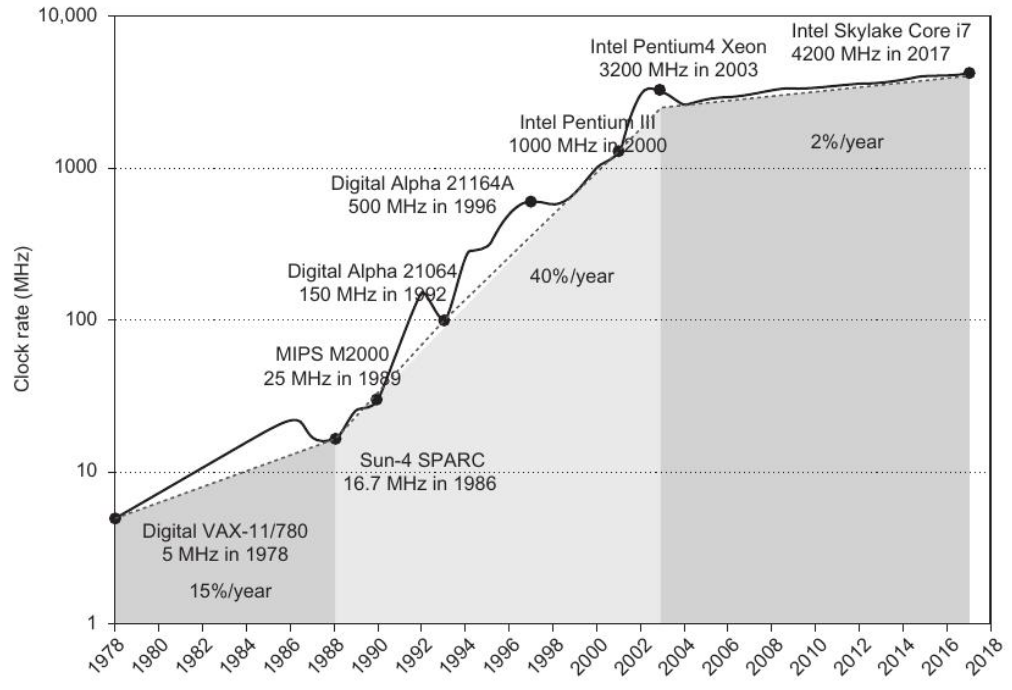
\includegraphics[width = 0.6\textwidth]{assets/power_issue.png}
\end{figure}

Roughly the capacitance and the voltage of transistor shrinks with the feature size, whereas the scaling is much more complicated for the wires.

Overall, a typical CPU got from ~2W power to ~100W which is at the limit of the air cooling capacity.

Primary strategies to cope with the power wall:

\begin{enumerate}
    \item Turn off inactive circuits (dark silicon)
    \item Downscale Voltage and Frequency for both cores and DRAM
    \item Thermal Power Design, or design for typical case
    \item Overclocking for a short period of time and possibly for just a fraction of the chip
\end{enumerate}

Static power, $Pstatic \propto Currentstatic \times V$, is also an important factor in the power consumption. It increases with the number of transistor while the current leakage increases as the feature size decreases and could amount to ~25\% of the total power consumption.

\subsubsection{Cache}

Another problem is the one colles the memory wall: the memory speed is not increasing as fast as the CPU speed, and the latency is not decreasing as fast as the CPU latency:

The CPU may spend more time waiting for data coming from RAM than executing ops.

The solution is to equip the CPU with a faster memory, that, by the way, is also way more expensive and way more energy consuming.

Furthermore, to be faster it ought to be extremely closer. All in all, the new memory that will be called cahce, will be much smaller then RAM.

We are quite naturally led to the "principle of locality":

Data are defined “local” when they reside in a “small”portion of the address space that is accessed in some “short” period of time

Local data are more likely to be in the cache.

\begin{itemize}
    \item \textbf{Temporal locality}: if a data is accessed, it is likely to be accessed again soon
    \item \textbf{Spatial locality}: if a data is accessed, it is likely that nearby data will be accessed soon
\end{itemize}

\subsubsection{Cache misses}

The cache is organized in lines, each line is a fixed number of bytes (e.g. 64 bytes) and each line is associated with a tag that identifies the memory address of the first byte of the line.

When the CPU needs to access a memory location, it first checks if the line containing that memory location is in the cache. If it is, it is a cache hit, otherwise it is a cache miss.

There are different types of cache misses:

\begin{itemize}
    \item \textbf{Compulsory miss}: Unavoidable misses when the cache is empty and the CPU needs to access a memory location for the first time
    \item \textbf{Capacity miss}: It occurs when there is not enaugh space to hold all data, or if there is too much data accessed in between successive use.
    \item \textbf{Conflict miss}: the cache is full and the CPU needs to evict a line to make space for the new one, but there is no other line that can be evicted
\end{itemize}

\subsubsection{Cache optimization}

It is possible to reduce the number of cache misses by:

\begin{itemize}
    \item \textbf{Rearrange (code and data)}: Design layout to improve temoral and spatial locality;
    \item \textbf{Reduce (size)}: Reduce the size of the data structures and the number of instructions;
    \item \textbf{Reuse (cache lines)}: Increase spatial and temporal locality, keep resident data in cache for more operations.
\end{itemize}
\section{Cache Mapping}

Modern systems subdivide both RAM and cache into equally sized blocks (often called \textit{lines}). For instance, a 64\,B block is commonly used: when a byte is requested, the entire 64\,B block containing that byte is fetched into the cache. This approach reduces the overhead of fetching data from memory and exploits spatial locality.

\begin{figure}[H]
    \centering
    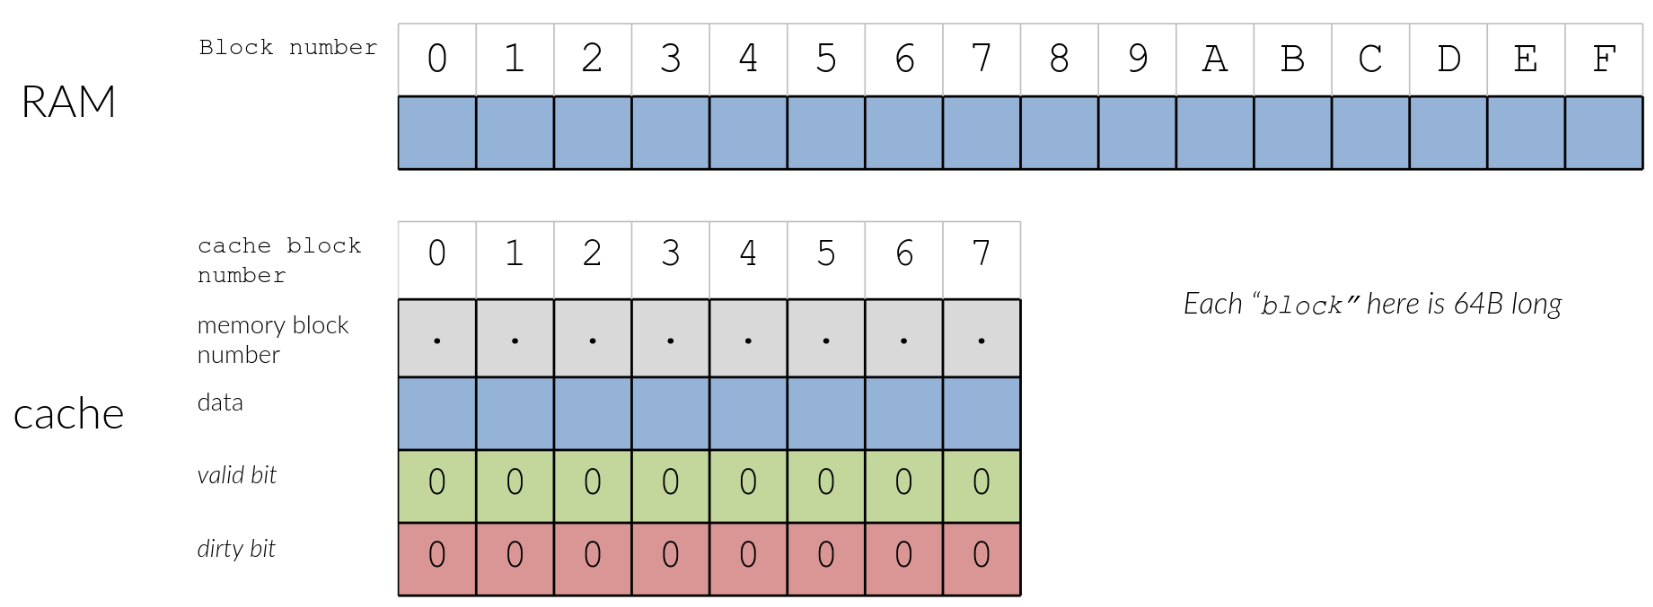
\includegraphics[width=0.8\textwidth]{assets/cache_mapping.png}
    \caption{Main memory and cache are both split into blocks (lines).}\label{fig:cache_mapping}
\end{figure}

There are three primary strategies for mapping main memory blocks into cache:

\begin{itemize}
    \item \textbf{Fully Associative Mapping}
    \item \textbf{Direct Mapping}
    \item \textbf{N-way (Set) Associative Mapping}
\end{itemize}

Each strategy differs in how flexible it is in placing a main memory block into cache and how it handles conflicts when multiple blocks compete for the same cache location. A high-level comparison is shown in \cref{fig:cache_mapping_ways}.

\begin{center}
    \begin{minipage}{0.2\textwidth}
        \centering
        \small
        \textbf{Fully Associative}
    \end{minipage}%
    \hspace{0.55em}
    \begin{minipage}{0.2\textwidth}
        \centering
        \small
        \textbf{Direct Mapping}
    \end{minipage}%
    \hspace{0.55em}
    \begin{minipage}{0.2\textwidth}
        \centering
        \small
        \textbf{N-way Associative}
    \end{minipage}
    \hspace{0.3em}
\end{center}

\vspace{-1em}

\begin{figure}[H]
    \centering
    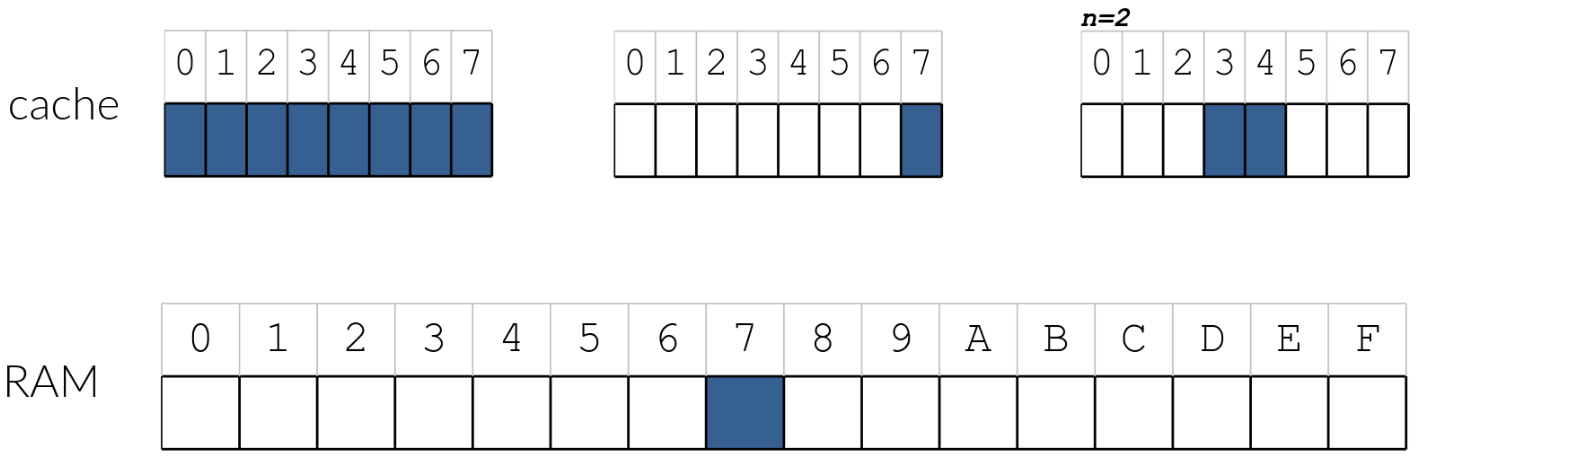
\includegraphics[width=0.77\textwidth]{assets/cache_mapping_ways.png}
    \caption{Fully Associative, Direct, and N-way Set Associative mappings.}\label{fig:cache_mapping_ways}
\end{figure}

\subsubsection{Fully Associative Mapping}
In a \textbf{fully associative} cache, each block of main memory \bfit{can be placed in any block} of the cache. This offers maximum flexibility because there is no restriction on which cache line a particular memory block can occupy. However, this scheme also requires more complex hardware for searching (to locate a given address in any cache line), making it more expensive.

\begin{minipage}[t]{0.48\textwidth}
    \textbf{Pros}
    \begin{itemize}
        \item Minimizes conflicts during \textit{writes}, as any free cache line can be used.
        \item Offers the greatest flexibility in block placement.
    \end{itemize}
\end{minipage}\hspace{1em}
\begin{minipage}[t]{0.48\textwidth}
    \textbf{Cons}
    \begin{itemize}
        \item Potentially inefficient for \textit{reads} because the requested data could be in any cache line, requiring a more expensive search mechanism (e.g., parallel or associative search).
        \item Higher hardware complexity and cost (larger tag comparators, fully associative lookups).
    \end{itemize}
\end{minipage}

\subsubsection{Direct Mapping}
In a \textbf{direct-mapped} cache, each block of main memory \bfit{can be placed in exactly one block} of the cache. This mapping is determined by some bits of the memory address (e.g., index bits), which directly select the cache line. It is the simplest scheme in terms of hardware.

\begin{minipage}[t]{0.48\textwidth}
    \textbf{Pros}
    \begin{itemize}
        \item Very efficient in locating or writing data because each memory block maps to a single known location (no associative search needed).
        \item Simpler and cheaper hardware implementation.
    \end{itemize}
\end{minipage}\hspace{1em}
\begin{minipage}[t]{0.48\textwidth}
    \textbf{Cons}
    \begin{itemize}
        \item Maximizes cache conflicts when multiple addresses map to the same cache line (known as \textit{conflict misses}).
        \item A single cache line might be heavily contended by multiple memory blocks, reducing overall hit rate.
    \end{itemize}
\end{minipage}

\subsubsection{N-way Set Associative Mapping}
In an \textbf{N-way set associative} cache, the cache is divided into sets, each containing $N$ lines. A block of main memory \bfit{can be placed in any of the $N$ lines} within the specific set dictated by the address. This approach strikes a balance between fully associative and direct-mapped schemes.


\begin{minipage}[t]{0.48\textwidth}
    \textbf{Pros}
    \begin{itemize}
        \item Reduces conflict misses compared to direct mapping by allowing multiple possible lines in each set.
        \item Lower hardware complexity than fully associative (search is limited to $N$ lines in the set, not the entire cache).
    \end{itemize}
\end{minipage}\hspace{1em}
\begin{minipage}[t]{0.48\textwidth}
    \textbf{Cons}
    \begin{itemize}
        \item More complex than direct mapping (requires searching up to $N$ lines in the set).
        \item Additional hardware and logic needed to manage the multiple lines per set.
    \end{itemize}
\end{minipage}

The choice of cache mapping strategy involves a trade-off between hardware complexity, access speed, and conflict rate.

\dots

